\documentclass[letterpaper,11pt]{article}

% Soporte para los acentos.
\usepackage[utf8]{inputenc}
\usepackage[T1]{fontenc}
% Idioma español.
\usepackage[spanish,mexico, es-tabla]{babel}
% Soporte de símbolos adicionales (matemáticas)
\usepackage{multirow}
\usepackage{amsmath}
\usepackage{amssymb}
\usepackage{amsthm}
\usepackage{amsfonts}
\usepackage{mathtools}
\usepackage{latexsym}
\usepackage{enumerate}
\usepackage{ragged2e}
\usepackage{listings}
\usepackage[dvipsnames]{xcolor}
\usepackage{graphicx}
\usepackage{hyperref}
\usepackage[linguistics]{forest}
\usetikzlibrary{positioning,matrix, arrows.meta}

% Modificamos los márgenes del documento.                                       
\usepackage[lmargin=1.5cm,rmargin=1.5cm,top=1.5cm,bottom=1.5cm]{geometry}

\title{Facultad de Ciencias, UNAM \\ 
       Análisis de Algoritmos \\ 
       Tarea 2 - Reposición}
\author{Rubí Rojas Tania Michelle}
\date{08 de enero de 2021}

\begin{document}
\maketitle

\begin{enumerate}
    % Ejercicio 1.
    \item Sea $M [1 \dots n][1 \dots n]$ una matrix de $n \times n$, en el que 
    cada renglón y cada columna están ordenados en orden creciente. Suponga que 
    no hay dos elementos iguales.
    
    \begin{enumerate}
        % Ejercicio 1.a
        \item Diseña un algoritmo que encuentre la posición de un valor $k$ en 
        $M$ o que determine si que no está. ¿Cuántas comparaciones usa tu 
        algoritmo en el peor caso?

        \textsc{Solución:} Como los elementos de las columnas y las filas 
        están ordenados de forma creciente, entonces podemos buscar el valor 
        de $k$ buscando en submatrices desde uno de los extremos, en 
        particular, desde el extremo superior derecho de la matriz. Usando la 
        información que nos proporciona la matriz, podemos encontrar un 
        camino que nos lleve al valor indicado. Esto se puede hacer con el 
        siguiente algoritmo:
        \begin{enumerate}
            \item Definimos \texttt{fila} $= 1$ y  \texttt{columna} $= n$.

            \item Mientras \texttt{fila} sea menor o igual a $n$ y 
            \texttt{columna} sea mayor que $0$, 
            hacemos:
            \begin{itemize}
                \item Si $M[fila][columna]$ = k, entonces regresamos la tupla 
                $(i,j)$.Terminamos.

                \item Si $M[fila][columna] < k$, entonces incrementamos en 
                una unidad el valor de \texttt{fila}.

                \item En otro caso, entonces disminuimos en una unidad el 
                valor de \texttt{columna}.
            \end{itemize}

            \item Si llegamos a este punto, es que no hemos encontrado el 
            valor del elemento que nos piden, por lo que simplemente regresamos 
            un $-1$. Terminamos. 
        \end{enumerate}

        Este algoritmo funciona porque en cada submatriz de tamaño $fila \times 
        columna$ garantizamos que está el elemento que buscamos. Como iniciamos 
        a comparar desde el elemento que está en la esquina superior derecha 
        de la matriz, entonces si hay un elemento mayor que él, éste debería 
        de estar en alguna de las filas que están abajo de él (ya que las 
        columnas y las filas están ordenadas). Pero si es menor que él, 
        entonces debería de estar en alguna de las columnas anteriores. 
        De acuerdo a esto, vamos actualizando nuestra posición (lo que implica 
        que iremos reduciéndo el tamaño de la submatriz donde debería de estar 
        el elemento que buscamos) y aplicamos el mismo razonamiento para los
        elementos en cada una de las nuevas posiciones hasta encontrar al 
        elemento deseado. 

        Ahora bien, en el peor caso, recorremos toda una fila y toda una 
        columna de la matriz para encontrar el valor que buscamos. Cada 
        uno de estos recorridos nos toma tiempo lineal, por lo que la 
        complejidad total del algoritmo será de $O(n) + O(n) = O(n)$. Usando 
        este mismo razonamiento, como la matriz es cuadrada, entonces a lo 
        más hacemos $2n-1$ comparaciones para buscar al elemento en el peor 
        caso.

        % Ejercicio 1.b
        \item Describe y analiza un algoritmo para resolver el siguiente 
        problema en tiempo lineal. Dados $4$ indices  $i, j, i', j'$ como 
        entrada, calcule el número de elementos de $M$ que son más pequeños que 
        $M[i][j]$ y más grandes que $M[i'][j']$.

        \textsc{Solución:} Primero, veamos cómo podemos calcular el número de 
        elementos de $M$ que son más pequeños que $M[i][j]$. Los elementos sobre 
        los cuales tenemos certeza de que son menores que $M[i][j]$ están en el 
        subarreglo de tamaño $i \times j$. A este número le restamos una unidad 
        para no considerar al propio elemento, por lo que tendremos $(i \times j) - 1$
        elementos que forzosamente son menores a $M[i][j]$ (esto se debe a que 
        los elementos de las filas y las columnas están ordenados de forma 
        creciente). Ahora bien, puede que existan más elementos que sean menores 
        que $M[i][j]$ y que se encuentren a su derecha y por encima de la fila 
        $i$ o a la izquierda y por debajo de la fila $i$. Para poder determinar 
        el número de elementos menores que $M[i][j]$ en este subarreglo, entonces 
        comparamos a $M[i][j]$ con cada $M[i-1][j+k]$, donde 
        $k \in \{1, 2, \ldots, (n-j)\}$. Entonces, mientras $j+k$ sea menor o 
        igual a $n$, hacemos 
        \begin{enumerate}
            \item Si $M[i-1][j+k] < M[i][j]$, eso significa que todos los 
            elementos anteriores a $M[i-1][j+k]$ dentro de esa columna deberían 
            de ser menores que $M[i][j]$, por transitividad. Así, tenemos $i-1$ 
            elementos adicionales que son menores que $M[i][j]$. Aumentamos en 
            una unidad el valor de $k$, para así movernos a la siguiente columna.

            \item En otro caso, tenemos que subir una fila más arriba para 
            verificar si los elementos anteriores a $M[i-1][j+k]$ dentro de esa
            columna son menores a $M[i][j]$.
            \begin{itemize}
                \item La suma de los elementos menores a $M[i][j]$ se realizará 
                de manera análoga al paso anterior, considerando los $i-m$ 
                elementos que fueron menores por transitividad, donde $m$ fue 
                el número de filas hacia arriba que tuvimos que subir para que 
                se cumpliera $M[i-m][j+k] < M[i][j]$.

                \item Si encontramos a un elemento $A[i-m][j+k] < M[i][j]$
                entonces sumamos $i-m$ elementos a nuestra cuenta y nos 
                movemos a la columna de la derecha, para realizar el 
                procedimiento del paso $1$, pero desde la posición actual donde
                nos encontramos y con los valores $i-m$, $j+k$ correspondientes.

                \item Si llegamos al primer elemento de la columna, y tenemos 
                que este elemento tampoco es menor que $M[i][j]$, eso significa 
                que ya no hay elementos más a la derecha que puedan ser menores 
                que $M[i][j]$, así que terminamos de buscar y nos quedamos con 
                la cuenta de los elementos que llevamos. 
            \end{itemize}

            \item Una vez que terminamos el ciclo del punto anterior, significa 
            que ya no podemos recorrer más la matriz (o que ya no debemos, por 
            el último punto del paso $2$). Así que terminamos y regresamos la 
            cuenta de los números menores a $M[i][j]$ que llevamos.
        \end{enumerate}

        De manera análoga, realizamos este procedimiento sobre $M[i+1][j-k]$ y
        nos vamos moviéndo hacia la izquierda y hacia abajo. Además, el número 
        de elementos lo contamos por columna y no por fila, es decir, $j-m$
        es el número que debemos sumar, donde $m$ es el número de columnas que 
        nos movimos hasta ese punto.

        Ahora, para poder encontrar la cantidad de elementos que son mayores que
        $M[i'][j']$, usaremos un algoritmo análogo al anterior. Así, hay 
        $(n-i') \times (n-j')$ elementos que son forzosamente menores al 
        elemento. Nuevamente, disminuimos una unidad para no contar al propio 
        elemento. Entonces, hay $(n-i') \times (n-j') - 1$ elementos que son 
        forzosamente mayores que $M[i'][j']$. Luego, puede que existan más 
        elementos que sean mayores que $M[i'][j']$ a su izquierda y por debajo 
        de la fila $i$ o a su derecha y por encima de la fila $i$. Para poder 
        determinar el número de elementos que son mayores que $M[i'][j']$ en 
        este subarreglo, entonces comparamos a $M[i'][j']$ con cada 
        $M[i'+1][j'-k]$, donde $k \in \{1, 2, \ldots, (n-j')\}$. Entonces, 
        mientras $j'-k$ sea mayor o igual a $1$, hacemos:  
        \begin{enumerate}
            \item Si $M[i'+1][j'-k] > M[i'][j']$, eso significa que todos los 
            elementos siguientes a $M[i'+1][j'-k]$ dentro de esa columna 
            deberían de ser mayores que $M[i'][j']$, por transitividad. Así, 
            tenemos $i'+1$ elementos adicionales que son mayores que $M[i'][j']$. 
            Disminuimos en una unidad el valor de $k$, para así movernos a la 
            columna anterior (una a la izquierda).

            \item En otro caso, tenemos que bajar una fila para verificar si los
            elementos siguientes a $M[i'+1][j'-k]$ dentro de esa columna son 
            mayores a $M[i']['j]$.
            \begin{itemize}
                \item La suma de los elementos mayores a $M[i'][j']$ se 
                realizará de manera análoga al paso anterior, considerando los 
                $i+m$ elementos que fueron mayores por transitividad, donde 
                $m$ es el número de filas hacia abajo que tuvimos que recorrer 
                para que se cumpliera $M[i'+m][j'-k] < M[i'][j']$.

                \item Si encontramos a un elemento $A[i'+m][j'-k] < M[i'][j']$
                entonces sumamos $i+m$ elementos a nuestra cuenta y nos movemos 
                a la columna de la izquierda para realizar el procedimiento del 
                paso $1$, pero desde la posición actual donde nos encontramos 
                y con los valores $i+m$, $j-k$ correspondientes.

                \item Si llegamos al último elemento de la columna, y tenemos 
                que este elemento tampoco es mayor que $M[i'][j']$, eso 
                significa que ya no hay elementos más a la izquierda que puedan 
                ser mayores que $M[i'][j']$, así que terminamos de buscar y nos 
                quedamos con la cuenta de los elementos que llevamos. 
            \end{itemize}

            \item Una vez que terminamos el ciclo del punto anterior, significa 
            que ya no podemos recorrer más la matriz (o que ya no debemos, por 
            el último punto del paso $2$). Así que terminamos y regresamos la 
            cuenta de los números menores a $M[i'][j']$ que llevamos.
        \end{enumerate}

        De manera similar, haremos este mismo procedimiento sobre $M[i-1][j+k]$
        y nos vamos moviéndo hacia la derecha y hacia arriba. Los elementos 
        que contamos son en dirección a las filas. 

        Este algoritmo funciona porque contemplamos todos las \textit{zonas} 
        o subarreglos cuyos elementos podrían ser menores (mayores) que 
        $M[i][j]$. Entonces, todo esto que contamos fueron las zonas que no 
        nos pedían, así que basta con hacer un resta de $n \times n$ con la
        suma total que arroja el algoritmo.

        Ahora bien, para encontrar la cantidad de elementos que son menores a 
        $M[i][j]$ sólo recorremos linealmente a la matriz, y en el peor de los
        casos tenemos que recorrer toda una columna y toda una fila; por lo que 
        la complejidad para obtener esta cantidad de elementos será $O(n)$. De 
        manera análoga, para encontrar la cantidad de elementos que son mayores 
        a $M[i'][j']$, el algoritmo toma tiempo lineal. Así, la complejidad 
        total del algoritmo nos tomará tiempo $O(n)$.
    \end{enumerate}
    
    % Ejercicio 2.
    \item {\bf Permutaciones de Josephus}: Supongamos que $n$ personas están 
    sentadas alrededor de una mesa circular con $n$ sillas, y que tenemos un
    entero positivo $m \leq n$. Comenzando con la persona con etiqueta $1$,
    (moviéndonos siempre el la dirección de las manecillas del reloj) comenzamos
    a remover los ocupantes de las sillas como sigue: Primero eliminamos la 
    persona con etiqueta $m$. Recursivamente, eliminamos al $m$-ésimo elemento 
    de los elementos restantes. Este proceso continua hasta que las $n$ personas 
    han sido eliminadas. El orden en que las personas han sido eliminadas, se 
    le conoce como la $(n, m)$-permutación de Josephus. Por ejemplo si $n=7$ y 
    $m=3$, la $(7,3)$-permutaci\'on de Josephus es: $\{3,6,2,7,5,1,4\}$.
         
    \begin{enumerate}
        % Ejercicio 2.a
        \item Supongamos que $m$ es constante. De un algoritmo lineal para generar
        la $(n,m)$-permutación de Josephus.

        \textsc{Solución:} Usaremos una lista circular para este caso. Las listas 
        circulares tienen las mismas propiedades que las listas ligadas, sólo se 
        añade que la cola y la cabeza están conectadas.

        Como tenemos $n$ personas alrededor de la mesa, entonces creamos una lista 
        circular \texttt{listaC} de longitud $n$, cuyos elementos son los enteros 
        $1, 2, 3, \ldots n$. Pero también necesitamos una lista vacía 
        \texttt{listaP} para ir agregando la $(n, m)$-permutación de Josephus, 
        así que también la creamos. Ahora lo que tenemos que hacer es encontrar 
        al $m-$ésimo elemento de \texttt{listaC} desde nuestra posición actual 
        (esto lo hacemos moviéndonos $m-1$ luagres desde donde estamos, e 
        iniciamos en la cabeza), lo agregamos a \texttt{listaP}, lo eliminamos
        de \texttt{listaC} y repetimos el proceso hasta que eliminemos a todos 
        los elementos de la lista. Esto se puede ver con el siguiente algoritmo:
        \begin{enumerate}
            \item Nos posicionamos en la cabeza de \texttt{listaC}.

            \item Si la longitud de \texttt{listaC} es igual a $1$, entonces 
            simplemente agregamos el elemento en la cabeza de \texttt{listaC} a
            \texttt{listaP}. 

            \item Avanzamos $m-1$ posiciones a la derecha de la lista para 
            encontrar al $m-$ésimo elemento de la lista (esto porque comenzamos 
            a contar a partir del siguiente elemento). Lo agregamos a 
            \texttt{listaP}, actualizamos nuestra posición actual en 
            \texttt{listaC} a la posición siguiente de donde estamos y eliminamos 
            al elemento anterior (que es el $m-$ésimo). Repetimos este proceso 
            (comenzando por el paso $2$) desde nuestra posición actual (que es 
            la posición siguiente del elemento que eliminamos) hasta que la 
            longitud de \texttt{listaC} sea igual a $1$ (pues ya sólo agregamos 
            a \texttt{listaP} al elemento que nos hace falta).

            \item Regresamos \texttt{listaP}.
        \end{enumerate}

        Este algoritmo funciona porque en cada iteración nos aseguramos de 
        encontrar al $m-$ésimo elemento e ir actualizando nuestra posición 
        correctamente. Como la lista es circular, entonces podemos ir 
        \textit{dando vueltas} en la lista y sólo nos vamos moviéndo $m-1$ 
        luagres para ir encontrando la posición deseada. Además, nos aseguramos
        de eliminar al $m-$ésimo elemento e ir actualizando nuestras referencias 
        adecuadamente. 

        Finalmente, crear a \texttt{listaC} nos toma tiempo lineal (ya que le 
        agregamos $n$ elementos) y crear a \texttt{listaP} nos toma tiempo 
        constante (pues es vacía). Como $m \in O(1)$, entonces movernos $m-1$ 
        posiciones a la derecha nos tomará también tiempo constante. Pero esto 
        lo hacemos $n-1$ veces, por lo que esto también nos cuesta tiempo lineal 
        en total. Agregar un elemento a \texttt{listaP} nos toma tiempo constante
        (pues lo estamos agregando al final). Y eliminar al elemento también nos 
        toma tiempo constante (pues siempre eliminamos al elemento anterior, y 
        para hacer esto sólo actualizamos las referencias de los nodos; por lo 
        que nunca recorremos la lista para poder eliminarlo), pero esto lo hacemos 
        también $n-1$ veces, por lo que en total nos toma tiempo lineal. Así, como 
        realizamos puras operaciones lineales a lo largo de este algoritmo, 
        entonces la complejidad total de éste es de $O(n)$.

        Un ejemplo para ilustrar el algoritmo sería el siguiente: si $n = 5$ y 
        $m = 4$, entonces
        \begin{figure}[h!]
        \centering
        \begin{tikzpicture}
            \matrix (A) [matrix of nodes, nodes={draw, minimum size=8mm},
                             column sep=-\pgflinewidth]{
            1 & 2 & 3 & \textcolor{blue}{4} & 5 \\};
        \end{tikzpicture}
        \caption{\texttt{listaC.cabeza.elemento = 1; $m-1 = 3$ y listaP = []}}
        \end{figure}

        \begin{figure}[h!]
        \centering
        \begin{tikzpicture}
            \matrix (A) [matrix of nodes, nodes={draw, minimum size=8mm},
                             column sep=-\pgflinewidth]{
            1 & 2 & 3 & \textcolor{red}{5} \\};
        \end{tikzpicture}
        \caption{\texttt{listaP = [4], posicionActual.elemento = 5}}
        \end{figure}
        
        \begin{figure}[h!]
        \centering
        \begin{tikzpicture}
            \matrix (A) [matrix of nodes, nodes={draw, minimum size=8mm},
                             column sep=-\pgflinewidth]{
            1 & 2 & \textcolor{blue}{5} \\};
        \end{tikzpicture}
        \caption{\texttt{listaP = [4, 3], posicionActual.elemento = 5}}
        \end{figure}

        \begin{figure}[h!]
        \centering
        \begin{tikzpicture}
            \matrix (A) [matrix of nodes, nodes={draw, minimum size=8mm},
                             column sep=-\pgflinewidth]{
            \textcolor{red}{1} & 2 \\};
        \end{tikzpicture}
        \caption{\texttt{listaP = [4, 3, 5], posicionActual.elemento = 1}}
        \end{figure}

        \begin{figure}[h!]
        \centering
        \begin{tikzpicture}
            \matrix (A) [matrix of nodes, nodes={draw, minimum size=8mm},
                             column sep=-\pgflinewidth]{
            \textcolor{blue}{1} \\};
        \end{tikzpicture}
        \caption{\texttt{listaP = [4, 3, 5, 2], posicionActual.elemento = 1}}
        \end{figure}

        \begin{figure}[h!]
        \centering
        \begin{tikzpicture}
            \matrix (A) [matrix of nodes, nodes={draw, minimum size=8mm},
                             column sep=-\pgflinewidth]{
            \textcolor{red}{1} \\};
        \end{tikzpicture}
        \caption{\texttt{listaC.length = 1 => listaP = [4, 3, 5, 2, 1] Terminamos}}
        \end{figure}
          
        % Ejercicio 2.b
        \item Supongamos que $m$ no es constante. Describa un algoritmo con
        complejidad $O(n \log n)$ para encontrar la $(n,m)$-permutación de 
        Josephus.

        \textsc{Solución:} Para este caso, utilizaremos un árbol binario 
        balanceado cuyas hojas tendrán como elemento a los enteros del conjunto 
        \{1, 2, \ldots, n\}, respectivamente; por lo que tendremos $n$ hojas. 
        Además, se debe cumplir que los nodos padres de las hojas tengan como 
        elemento el número de hojas que tienen. El resto de los nodos internos 
        tendrán como elemento el número de hojas que tienen sus dos subárboles
        (cada nodo obtiene esto sumando los elementos que tienen sus nodos 
        hijos, pues desde la propiedad anterior estamos garantizando que los 
        padres de las hojas nos proporcionan esta información).
        La construcción de este árbol la haremos de abajo hacia arriba, y será 
        como sigue:
        \begin{itemize}
            \item Construimos $n$ hojas cuyos elementos son $1, 2, \ldots, n$;
            respectivamente. Además, los marcamos como no visitados.

            \item Para crear los padres de las hojas:
            \begin{itemize}
                \item Calculamos \texttt{altura} $= \lceil \log(n)\rceil$ + 1. 
    
                \item Tomamos el primer par de hojas (de izquierda a derecha) y 
                construimos al nodo padre. Éste tendrá como elemento al número 
                $2$, ya que tiene dos hojas.
    
                \item Después, tomamos el siguiente par de hojas y realizamos el 
                paso anterior. 
                
                \item Si al momento de querer tomar un par de nodos tenemos que 
                sólo podemos tomar uno, es decir, sólo queda o sólo hay una hoja 
                en el nivel, entonces construimos al nodo padre y su elemento 
                será el número $1$, pues sólo tiene una hoja. Pasamos al
                siguiente punto del algoritmo.

                \item Si al momento de querer tomar un par de nodos tenemos que 
                ya no hay nodos (es decir, el número de hojas era par), entonces 
                pasamos al siguiente punto del algoritmo.
            \end{itemize}

            \item Una vez que terminamos de construir los nodos padre de las
            hojas, disminuimos en uno la variable \texttt{altura}.

            \item Para crear los nodos internos faltantes:

            Mientras \texttt{altura} sea mayor que $1$, hacemos lo siguiente 
            para los últimos nodos padres que hayamos creado (la primera 
            iteración es sobre los padres de las hojas, después será sobre 
            los padres de los padres de las hojas y así sucesivamente); 
            \begin{itemize}
                
                \item Tomamos los primeros dos nodos y construimos el nodo 
                padre. El elemento del padre tendrá la suma de los elementos 
                de sus hijos, por lo que \\ 
                \texttt{padre.elemento = padre.izquierdo.elemento + 
                padre.derecho.elemento}.
    
                \item Después tomamos el siguiente par de nodos y realizamos 
                el paso anterior. 
                
                \item Si al momento de querer tomar un par de nodos sólo podemos 
                tomar uno, es decir, sólo queda un nodo en el nivel, entonces 
                construimos un nodo padre, y tendrá como hijos a este último nodo 
                y al último nodo padre que construimos. El elemento de este 
                nuevo nodo padre será la suma de los elementos de sus hijos. 
                Disminuimos en una unidad a la variable \texttt{altura} y 
                volvemos a repetir el proceso, pero ahora sobre los nuevos nodos 
                padres que hemos creado.

                \item Si al momento de querer tomar un par de nodos tenemos 
                que ya no hay nodos (es decir, el número de nodos era par), 
                entonces disminuimos en una unidad a la variable \texttt{altura}
                y volvemos a repetir el proceso, pero ahora sobre los nuevos 
                nodos padres que hemos creado. 
            \end{itemize}

            \item Cuando llegamos a que \texttt{altura} es menor o igual a $1$, 
            significa que ya construimos la raíz del árbol. Terminamos.
        \end{itemize}

        Ahora necesitamos una forma de recorrer el árbol de tal forma que 
        podamos encontrar cualquiera de las $m$ posiciones que necesitemos 
        buscar. Para buscar nuestra hoja, nos apoyaremos de la información 
        que contiene cada uno de nuestros nodos internos. Cada nodo conoce 
        el número de elementos de $n$ que contiene cada uno de sus subárboles, 
        así que usando esto podemos determinar, estando desde la raíz del árbol, 
        hacia cuál de los subárboles debemos movernos. Este proceso lo hacemos 
        recursivamente (desde la raíz de los subárboles) hasta que encontramos 
        la hoja que necesitamos. 
        
        Esto se puede ver con el siguiente algoritmo:
        \begin{enumerate}
            \item Nos posicionamos en la raíz del árbol y hacemos 
            \texttt{nodo = raiz}.

            \item Mientras el hijo izquierdo del \texttt{nodo} no sea una 
            hoja, hacemos:
            \begin{itemize}
                \item Si $m$ es menor o igual al elemento del hijo izquierdo 
                del \texttt{nodo}, entonces nos movemos al subárbol izquierdo 
                de éste, es decir, \texttt{nodo = nodo.hijoIzquierdo}.

                \item En otro caso, actualizamos el valor de $i$ como 
                $m = m -$ \texttt{nodo.hijoIzquierdo.elemento}, y nos movemos 
                al subárbol derecho; es decir, \texttt{nodo = nodo.hijoDerecho}.
            \end{itemize}

            \item Para este punto, los hijos del \texttt{nodo} serán ambos 
            hojas (si es que tiene dos). Así que tenemos dos opciones:
            \begin{itemize}
                \item Si $m$ es igual a $1$ pero el hijo izquierdo ya ha sido 
                visitado, entonces nos movemos a la hoja derecha; es decir, 
                \texttt{nodo = nodo.hijoDerecho}.

                \item Si $m$ es igual a $1$, entonces nos movemos a la 
                hoja izquierda; es decir, \\ 
                \texttt{nodo = nodo.hijoIzquierdo}. Marcamos como visitada a 
                la hoja. Terminamos.

                \item En otro caso, nos movemos a la hoja derecha; es decir, 
                \texttt{nodo = nodo.hijoDerecho}. Marcamos como visitada a la 
                hoja. Terminamos. 
            \end{itemize}
        \end{enumerate}

        Una vez que tenemos una forma de buscar en el árbol, ya podemos comenzar 
        a buscar la $(n-m)$ permutación de Josephus. Iniciamos en la primer 
        posición, que sería el número $1$. Le sumamos $(m-1)$ (para poder obtener 
        la $m-$ ésima posición) y lo buscamos en el árbol. Una vez que lo encontramos, 
        guardamos el valor de su elemento en una lista y lo eliminamos. Actualizamos 
        nuestras referencias (la próxima posición inicial es la posición siguiente del 
        elemento que eliminamos) y repetimos este proceso hasta que hayamos eliminado 
        a todos los elementos en el árbol.

        El algoritmo entero sería como:
        \begin{enumerate}
            \item Construimos el árbol con las $n$ hojas y creamos una lista 
            vacía \texttt{listaP}.

            \item Definimos \texttt{posicion = 1}, un contador $i = 1$ y 
            \texttt{len = n}.

            \item Mientras $i$ sea menor o igual que \texttt{len}:
            \begin{itemize}
                \item Calculamos \texttt{posicion = posicion + (m-1)}

                \item Si $n$ es menor que \texttt{posicion} entonces 
                actualizamos el valor de la posición como 
                \texttt{posicion = ((posicion-1) \% n) + 1} 

                \item Buscamos a \texttt{posicion} en el árbol. Una vez 
                que estemos en la hoja correspondiente, guardamos el valor 
                de la hoja en \texttt{listaP} y \textit{eliminamos} al elemento:
                siguiendo el mismo camino que recorrió nuestro algoritmo de 
                búsqueda, vamos a disminuir en una unidad el valor de todos los 
                nodos visitados durante la búsqueda. 

                \item Disminuimos en una unidad a $n$ e incrementamos en una 
                unidad al contador $i$.
            \end{itemize}

            \item Regresamos \texttt{listaP}. Terminamos.
        \end{enumerate}

        El algoritmo funciona por cómo está construido el árbol y porque gracias 
        a las operaciones que realizamos, podemos obtener correctamente al 
        $m-$ ésimo elemento y mantener actualizadas nuestras referencias. El 
        árbol está construido de tal forma que los nodos internos nos 
        proporcionen información valiosa para hacer la búsqueda de elementos 
        hojas en el árbol (cada nodo sabe cuántas hojas contienen sus dos 
        subárboles). La búsqueda de elementos en el árbol funciona correctamente 
        gracias a que en cada iteración garantizamos que el subárbol en el que 
        nos posicionamos contiene al $m-$ésimo elemento (como los nodos contienen 
        el número de hojas que tiene cada uno de sus subárboles, entonces así 
        podemos decidir a cuál subárbol movernos, y cada vez que nos movemos al 
        subárbol derecho, actualizamos el valor de la posición que buscamos). 
        Al momento de eliminar, basta con que borremos todas las referencias 
        que indican que en esa hoja hay un elemento. Así, al momento de buscar 
        nuevamente otro elemento en el árbol, gracias a cómo lo hace, podemos 
        ignorar los subárboles donde no hay elementos y además como actualizamos 
        parte del árbol (el recorrido de la hoja hacia la raíz), entonces siempre 
        mantenemos las referencias actualizadas para poder saber cuántas hojas 
        tiene cada subárbol. Luego, para calcular la $m-$ésima posición, damos 
        $m-1$ saltos para poder encontrar la siguiente posición a eliminar. En 
        dado caso de que la suma que realicemos esté fuera del rango $n$, 
        tenemos que calcular \texttt{((posicion-1) \% n) + 1} para poder 
        regresar nuestro valor de nuevo al rango $n$ y que además sea el 
        correcto. Así que por esto podemos garantizar que las referencias están 
        siempre actualizadas y que siempre vamos a poder calcular la $m-$ésima 
        posición correctamente.

        Ahora bien, notemos que construir el árbol nos toma $O(n)$ ya que lo 
        estamos construyendo de abajo hacia arriba, y progresivamente vamos 
        formando los $n-1$ nodos internos. Crear la lista vacía nos toma tiempo 
        constante. Buscar al $m-$ésimo elemento nos toma $O(\log n)$ ya que en 
        el peor de los casos recorremos la altura del árbol (pues los elementos 
        que buscamos son hojas), pero esto lo hacemos $n$ veces, por lo que nos 
        toma $O(n \log n)$ esta operación en total. La operación eliminar no 
        elimina nodos del árbol, lo único que hace es borrar las referencias 
        de él en el árbol al disminuir en una unidad todos los elementos en los 
        nodos visitados al momento de buscar la hoja (hacemos como que no 
        existe). Entonces, tenemos que recorrer en el peor de los casos la 
        altura del árbol, por lo que nos toma tiempo $O(\log n)$. Pero, esta 
        operación la realizamos $n$ veces, así que en total nos toma tiempo 
        $O(n \log n)$. El resto de las operaciones que realizamos son constantes, 
        pues sólo hacemos asignaciones. Por lo tanto, la complejidad total del 
        algoritmo es de $O(n \log n)$.

        Un ejemplo para ilustrar la construcción del árbol y la búsqueda de 
        un elemento sería el siguiente: si $n=5$ (tenemos $5$ hojas) y 
        buscamos al elemento $3$, entonces el árbol se vería como
        \begin{figure}[h!]
        \centering
        \forestset{default preamble={for tree={circle,draw}}}
        \begin{forest}
        [5, red
          [4, red 
            [2 [1] [2]] 
            [2, red [3, blue] [4]]] 
          [1 [5]]]
        \end{forest}
        \caption{En color \textcolor{red}{rojo} está el camino a seguir para 
                 encontrar al elemento $3$}
        \end{figure}
    \end{enumerate}
         
    % Ejercicio 3.
    \item Queremos ordenar una lista $S$ de $n$ enteros que contiene muchos 
    elementos duplicados. Supongamos que los elementos de $S$ sólo toman 
    $O(\log n)$ valores distintos.

    \begin{itemize}
        % Ejercicio 3.a
        \item Encuentre un algoritmo que toma a lo más $O(n \log \log n)$ tiempo 
        para ordenar S.

        \textsc{Solución:} Para este caso, vamos a utilizar un árbol $AVL$, ya 
        que éste es un árbol binario de búsqueda que está balanceado. La única 
        propiedad que le vamos a agregar es que cada nodo contiene el valor de 
        su elemento y su número de repeticiones en el arreglo. La construcción 
        del árbol será como sigue:
        \begin{enumerate}
            \item Definimos el árbol $T = \varnothing$.

            \item Definimos \texttt{nodo = S.cabeza}.
            
            \item Mientras \texttt{nodo != null}, hacemos:
            \begin{itemize}
                \item Si el elemento en el \texttt{nodo} ya se encuentra en el 
                árbol $T$, entonces no lo agregamos, simplemente aumentamos el 
                contador en una unidad en su nodo correspondiente, es decir,
                \texttt{nodo.repeticiones += 1} 

                \item En caso contrario, agregamos el elemento al árbol y 
                definimos su contador de repeticiones en 1, es decir, 
                \texttt{nodo.repeticiones = 1}.

                \item Pasamos al elemento siguiente en la lista $S$, es decir, 
                \texttt{nodo = nodo.siguiente}.
            \end{itemize}
        \end{enumerate}

        Así, tenemos un árbol binario balanceado $T$ con un máximo de 
        $\log n$ nodos distintos en el árbol. Por lo tanto, la altura máxima 
        de $T$ será de $\log (\log n)$. Como el árbol es de búsqueda, entonces 
        basta con que recorramos el árbol en forma in-order para obtener al 
        arreglo ordenado. Creando una lista $A$ podemos ir guardando los 
        elementos que vayamos visitando en el árbol cuando lo recorremos, y de 
        acuerdo al contador de repeticiones en el nodo, sabremos cuantas veces 
        debemos copiar este elemento en la lista $A$. Finalmente, regresamos
        la lista $A$.

        Este algoritmo funciona porque gracias a las operaciones del árbol 
        AVL podemos guardar correctamente a los $n$ elementos de la lista 
        $S$ y contar las apariciones de éstos. Notemos que la operación 
        agregar hace los giros necesarios para que el árbol siga balanceado.
        Una vez que el árbol se haya creado, entonces el recorrido in-order 
        nos garantiza obtener a los elementos ordenados (por como está 
        definido un árbol de búsqueda), y el contador de repeticiones sólo nos 
        indica cuántas veces hay que copiar ese elemento en la lista $A$.
        Así, podemos obtener correctamente a la lista ordenada.

        Ahora bien, la verificación de que un elemento ya está en el árbol se 
        realiza en el mismo algoritmo para insertar. Si el elemento que vamos 
        a agregar es igual a un nodo que visitamos durante la búsqueda del 
        lugar donde debemos posicionarlo, entonces simplemente aumentamos en 
        una unidad al contador del nodo correspondiente. En el peor de los 
        casos, para agregar (o verificar) un nodo al árbol tenemos que recorrer 
        toda la altura del árbol, que es $\log (\log n)$, por lo que esta 
        operación nos tomará $O(\log (\log n))$. Pero esta operación la 
        realizamos para cada uno de los $n$ elementos de la lista $S$, por lo 
        que nos tomará $O(n \log (\log n))$ tiempo. Además, el recorrer el 
        árbol de forma in-order nos cuesta $O(n)$ y llenar la lista $A$ también 
        nos cuesta $O(n)$, por lo que la complejidad total del algoritmo será 
        de 
        \begin{equation*}
            O(n \log (\log n)) + O(n) + O(n) = O(n \log (\log n))
        \end{equation*}

        % Ejercicio 3.b
        \item ¿Por qué esto no viola la cota inferior de $O(n \log n)$ para el 
        problema de ordenación?

        \textsc{Solución:} La cota inferior para ordenar es para $n$ elementos 
        distintos usando comparaciones, y si un algoritmo de ordenamiento lo 
        usamos con $n$ elementos distintos, entonces necesariamente es 
        $O(n \log n)$. En este caso, tenemos información extra que nos da una 
        característica de los elementos (que su valor es a lo más $\log n$), 
        pero sobre ordenar no sabemos nada. En particular tenemos $\log n$
        elementos distintos, pero si fueran $n$ distintos entonces la 
        complejidad del algoritmo sería de $O(n \log n)$. Por este motivo,
        no viola la cota inferior para el problema de ordenación.
    \end{itemize}
    
    % Ejercicio 4.
    \item Dado un arreglo $A$ de $n$ números, queremos contestar la pregunta 
    ¿Hay algún elemento de $A$ que aparezca al menos $\frac{n}{3}$ veces? 
    Encuentre un algoritmo lineal para resolver este problema.

    \textsc{Solución:} Primero, necesitamos encontrar los elementos que son  
    candidatos a que se repitan $\frac{n}{3}$ veces. A lo más podemos tener 
    $3$ candidatos, pues en caso de que éstos se repitan $\frac{n}{3}$ veces, 
    entonces obtenemos el tamaño completo del arreglo. Así, creamos un arreglo 
    auxiliar $B$ de tamaño $3$. La estrategia es recorrer el arreglo $A$ una 
    primera vez para poder encontrar a los candidatos. Esto se hará como
    sigue:
    \begin{itemize}
        \item Definimos los contadores $cc_1 = cc_2 = cc_3 = 0$. A cada uno 
        de estos contadores le corresponde una entrada del arreglo $B$,
        respectivamente.

        \item Definimos un contador $i = 3$ para recorrer el arreglo.

        \item Agregamos a los tres primeros elementos de $A$ al arreglo $B$ y 
        aumentamos en una unidad a los tres contadores $cc$.
        
        \item Mientras $i < n$, hacemos:
        \begin{itemize}
            \item Si A[i] es igual a uno de los elementos de $B$, entonces 
            aumentamos su respectivo contador.

            \item En caso contrario, le restamos una unidad a todos nuestros 
            contadores $cc$ y colocamos a $A[i]$ en cualquier posición del arreglo 
            $B$ cuyo contador sea igual a $0$. 
        \end{itemize}
    \end{itemize}

    Una vez que tenemos a nuestros candidatos, entonces le cambiamos el valor a 
    nuestras variables $cc$ (ya que el valor que tenían antes ya no importa):
    \begin{equation*}
        c_1 = B[0] \quad \quad c_2 = B[1] \quad \quad c_3 = B[2]
    \end{equation*} 
    
    las cuales tendrán ahora los valores de cada uno de nuestros candidatos. 
    Así, basta con recorrer el arreglo $A$ como sigue:
    \begin{itemize}
        \item Definimos una variable $i=0$ para recorrer el arreglo.

        \item Mientras $i < n$, hacemos:
        \begin{itemize}
            \item Si A[i] es igual a $c_1$, entonces aumentamos en una unidad 
            al contador $cc_1$.

            \item Si A[i] es igual a $c_2$, entonces aumentamos en una unidad 
            al contador $cc_2$.

            \item Si A[i] es igual a $c_3$, entonces aumentamos en una unidad 
            al contador $cc_3$.
        \end{itemize}
    \end{itemize}

    Si hay algún contador $cc$ que sea igual a $\frac{n}{3}$, entonces 
    regresamos \texttt{true}. En caso contrario, regresamos \texttt{false}.

    El algoritmo funciona porque garantizamos que el arreglo auxiliar $B$ 
    contendrá al elemento que se repite $\frac{n}{3}$ veces. Esto se debe a 
    que si existe tal elemento, entonces debería de aparecer un número 
    suficiente de veces para que el arreglo lo guarde. Es decir, la primera 
    parte del algoritmo se encarga de buscar a los elementos que se repiten 
    más. Si un elemento se repite una cantidad \textit{significativa} de 
    veces, entonces al momento de restar una unidad a los contadores, 
    este elemento no podrá ser eliminado; o bien, si es eliminado, 
    eventualmente volverá a guardarse en $B$. Así, podemos estar seguros 
    de que guardamos al menos a un elemento que cumple la propiedad solicitada.

    Ahora bien, encontrar a los elementos candidatos nos cuesta 
    $3 \cdot O(n) = O(n)$, pues en el peor de los casos debemos recorrer todo 
    el arreglo auxiliar $B$ (de tamaño $3$) $n$ veces. Luego, recorremos 
    todo el arreglo $A$ para poder contar el número de apariciones de los 
    candidatos, y eso nos toma tiempo lineal. El resto de las operaciones nos 
    toman timpo constante. Por lo tanto, la complejidad total del algoritmo es 
    de $O(n) + O(n) = O(n)$.

    % Ejercicio 5.
    \item Sea $A[1, \ldots , n]$ un arreglo de números reales. Diseña un 
    algoritmo que realice cualquier secuencia de las siguientes operaciones:

	\begin{itemize}
        % Ejercicio 5.a
        \item $Add(i, y)$,  suma el valor $y$ al $i$-ésimo número.

        \textsc{Solución:} Sea $n$ la longitud del arreglo $A$. Para ejecutar
        esta operación, primero realizaremos un preprocesamiento de la 
        información. Lo que haremos será construir un árbol binario balanceado 
        donde las hojas de éste tendrán como elementos a los números reales de 
        $A$ (sin cambiar su órden de aparición). Además, se debe cumplir que 
        los nodos padres de las hojas tengan como elemento el número de hojas 
        que tienen. El resto de los nodos internos tendrán como elemento el 
        número de hojas que tienen sus dos subárboles (cada nodo obtiene esto 
        sumando los elementos que tienen sus nodos hijos, pues desde la 
        propiedad anterior estamos garantizando que los padres de las hojas nos 
        proporcionan esta información). La construcción de éste árbol la haremos 
        de abajo hacia arriba, y será como sigue:
        \begin{itemize}
            \item Construimos $n$ hojas cuyos elementos serán los elementos del 
            arreglo $A$, es decir, los elementos $A[1], A[2], \ldots, A[n]$.

            \item Para crear los padres de las hojas:
            \begin{itemize}
                \item Calculamos \texttt{altura} $= \lceil \log(n)\rceil$ + 1. 
    
                \item Tomamos el primer par de hojas (de izquierda a derecha) y 
                construimos al nodo padre. Éste tendrá como elemento al número 
                $2$, ya que tiene dos hojas.
    
                \item Después, tomamos el siguiente par de hojas y realizamos el 
                paso anterior. 
                
                \item Si al momento de querer tomar un par de nodos tenemos que 
                sólo podemos tomar uno, es decir, sólo queda o sólo hay una hoja 
                en el nivel, entonces construimos al nodo padre y su elemento 
                será el número $1$, pues sólo tiene una hoja. Pasamos al
                siguiente punto del algoritmo.

                \item Si al momento de querer tomar un par de nodos tenemos que 
                ya no hay nodos (es decir, el número de hojas era par), entonces 
                pasamos al siguiente punto del algoritmo.
            \end{itemize}

            \item Una vez que terminamos de construir los nodos padre de las
            hojas, disminuimos en uno la variable \texttt{altura}.

            \item Para crear los nodos internos faltantes:

            Mientras \texttt{altura} sea mayor que $1$, hacemos lo siguiente 
            para los últimos nodos padres que hayamos creado (la primera 
            iteración es sobre los padres de las hojas, después será sobre 
            los padres de los padres de las hojas y así sucesivamente); 
            \begin{itemize}
                \item Tomamos los primeros dos nodos y construimos el nodo 
                padre. El elemento del padre tendrá la suma de los elementos 
                de sus hijos, por lo que \\ 
                \texttt{padre.elemento = padre.izquierdo.elemento + 
                padre.derecho.elemento}.
    
                \item Después tomamos el siguiente par de nodos y realizamos 
                el paso anterior. 
                
                \item Si al momento de querer tomar un par de nodos sólo podemos 
                tomar uno, es decir, sólo queda un nodo en el nivel, entonces 
                construimos un nodo padre, y tendrá como hijos a este último nodo 
                y al último nodo padre que construimos. El elemento de este 
                nuevo nodo padre será la suma de los elementos de sus hijos. 
                Disminuimos en una unidad a la variable \texttt{altura} y 
                volvemos a repetir el proceso, pero ahora sobre los nuevos nodos 
                padres que hemos creado.

                \item Si al momento de querer tomar un par de nodos tenemos 
                que ya no hay nodos (es decir, el número de nodos era par), 
                entonces disminuimos en una unidad a la variable \texttt{altura}
                y volvemos a repetir el proceso, pero ahora sobre los nuevos 
                nodos padres que hemos creado. 
            \end{itemize}

            \item Cuando llegamos a que \texttt{altura} es menor o igual a $1$, 
            significa que ya construimos la raíz del árbol. Terminamos.
        \end{itemize}

        Sabemos que un árbol puede implementarse en un arreglo, así que este 
        procedimiento se realizará dentro de uno para ocupar el arreglo que se 
        nos permite usar como espacio extra. 
        
        Una vez que tengamos el árbol construido, entonces debemos recorrerlo de 
        tal forma que lleguemos al $i-$ésimo elemento de $A$, para luego sumarle 
        el valor de $y$. Esto lo podemos lograr realizando el siguiente 
        algoritmo:
        \begin{enumerate}
            \item Nos posicionamos en la raíz del árbol y hacemos 
            \texttt{nodo = raiz}. 

            \item Mientras el hijo izquierdo del \texttt{nodo} no sea una 
            hoja, hacemos:
            \begin{itemize}
                \item Si $i$ es menor o igual al elemento del hijo izquierdo 
                del \texttt{nodo}, entonces nos movemos al subárbol izquierdo 
                de éste, es decir, \texttt{nodo = nodo.hijoIzquierdo}.

                \item En otro caso, actualizamos el valor de $i$ como 
                $i = i -$ \texttt{nodo.hijoIzquierdo.elemento} y nos movemos 
                al subárbol derecho; es decir, \texttt{nodo = nodo.hijoDerecho}.
            \end{itemize}

            \item Para este punto, los hijos del \texttt{nodo} serán ambos 
            hojas (si es que tiene dos). Así que tenemos dos opciones:
            \begin{itemize}
                \item Si $i$ es igual a $1$, entonces nos movemos a la 
                hoja izquierda; es decir, \\ 
                \texttt{nodo = nodo.hijoIzquierdo}.

                \item En otro caso, nos movemos a la hoja derecha; es decir, 
                \texttt{nodo = nodo.hijoDerecho}.
            \end{itemize}

            \item Al elemento de \texttt{nodo} le sumamos el valor $y$. 
            Terminamos. 
        \end{enumerate}

        Este algoritmo funciona porque en cada iteración siempre garantizamos 
        estar en el subárbol donde se encuentra el $i-$ésimo elemento. Primero 
        nos posicionamos en la raíz del árbol, y la variable \texttt{nodo} nos 
        ayuda a mantener la referencia sobre el nodo en el que estamos 
        posicionados en este momento. Luego hacemos un recorrido entre los
        nodos internos hasta que llegamos a uno donde su hijo izquierdo es 
        una hoja (sólo verificamos al hijo izquierdo, por que un nodo interno 
        puede tener uno o dos hijos, y si sólo tiene uno, entonces será el 
        izquierdo). Durante este recorrido tenemos dos casos: nos movemos al 
        subárbol izquierdo o al subárbol derecho. Para tomar esta decisión, 
        debemos comparar al elemento del hijo izquierdo del nodo donde estamos 
        posicionados con nuestro índice $i$. Como los nodos internos 
        \textit{saben} cuántos elementos de $A$ tienen sus subárboles, 
        entonces si $i$ es menor o igual a \texttt{nodo.hijoIzquierdo.elemento}
        eso quiere decir que el elemento $i$ se encuentra dentro del rango 
        de elementos que contiene el subárbol izquierdo de \texttt{nodo}. En 
        caso contrario, debe estar en el subárbol derecho de \texttt{nodo}. 
        Pero, si nos movemos al subárbol derecho debemos de actualizar el 
        valor de $i$, así que le restamos el número de elementos de $A$ donde 
        sabemos que $i$ no va a estar (esto para que tenga el valor adecuado 
        respecto al nuevo subárbol con el que vamos a tratar). Una vez que 
        encontramos al nodo interno cuyos hijos (si es que tiene dos) son 
        hojas, entonces tenemos dos opciones: elegir la hoja izquierda o la 
        derecha. Esta decisión la tomaremos dependiéndo del valor que tenga 
        $i$ en ese momento. Si $i$ es igual a $1$ entonces el elemento que 
        buscamos está en la hoja izquierda. En caso contrario, el elemento que 
        buscamos está en la hoja derecha. Por los cambios que sufre $i$ en el 
        recorrido de nodos internos, entonces los valores finales que puede 
        tomar $i$ son $1$ o $2$; así que dependiéndo de esto, decidimos la 
        hoja que le corresponde. Finalmente, como encontramos la hoja que
        contiene al $i-$ésimo elemento de $A$, simplemente le sumamos el 
        valor de $y$ y terminamos. 

        La construcción del árbol nos toma $O(n)$ en tiempo y en espacio (ya 
        que lo construimos de abajo hacia arriba y progresivamente vamos 
        formando los $n-1$ nodos internos). Luego, como los elementos del 
        arreglo $A$ se encuentran en las hojas, entonces en el peor de los 
        casos tenemos que recorrer la altura del árbol para encontrar al 
        elemento que deseamos. Y como sumar el elemento $y$ con el elemento 
        encontrado nos toma tiempo constante, entonces la complejidad total 
        del algoritmo de búsqueda es de $O(\log n)$.

        Un ejemplo para ilustrar el algoritmo sería el siguiente: si 
        $A = [7, 14, 2, 8, 9, 11, 0, -1, 1]$ y \texttt{Add(7,6)}, entonces 
        \begin{figure}[h!]
        \centering
        \forestset{default preamble={for tree={circle,draw}}}
        \begin{forest}
        [9, red
          [4, 
            [2 
              [7] 
              [14]]
            [2 
              [2]
              [8]]]
          [5, red, edge label={node[midway,right,font=\scriptsize]{\;\;\;\;\;\; 
                                                                   i=7-4=3}}
            [4, red, edge label={node[midway,left,font=\scriptsize]{\; i=3}}
              [2
                [9] 
                [11]]
              [2, red, edge label={node[midway,right,font=\scriptsize]{\;\;i=3-2=1}}
                [6, blue]
                [-1]]]
            [1 
              [1]]]]
        \end{forest}
        \caption{En color \textcolor{red}{rojo} está el recorrido para llegar
                 al elemento $i=7$.}
        \end{figure}
        
        % Ejercicio 5.b
        \item $Partial-sum(i)$, regresa la suma de los primeros $i$ números, 
        es decir, 

        $Partial-sum(i) = A[1] + \ldots + A[i]$

        \textsc{Solución:} Usaremos básicamente el árbol del inciso anterior 
        para el preprocesamiento de la información, sólo le agregaremos la 
        propiedad de que cada nodo tiene una llave. La llave de las hojas 
        será el valor de su elemento. Las llaves de los nodos padre de las 
        hojas será la suma de las llaves de sus hijos. Las llaves de los 
        demás nodos internos serán la suma de las llaves de sus subárboles 
        (cada nodo obtiene esto sumando las llaves que tienen sus hijos, 
        pues desde la propiedad anterior estamos garantizando que los padres 
        de las hojas nos proporcionan esta información). La construcción
        de éste árbol la haremos de abajo hacia arriba, y será como sigue:
        \begin{itemize}
            \item Construimos $n$ hojas cuyos elementos serán los elementos del 
            arreglo $A$, es decir, los elementos $A[1], A[2], \ldots, A[n]$.
            El valor de las llaves de las hojas será el mismo que el valor de 
            su elemento. 

            \item Para crear los padres de las hojas:
            \begin{itemize}
                \item Calculamos \texttt{altura} $= \lceil \log(n)\rceil$ + 1. 
    
                \item Tomamos el primer par de hojas (de izquierda a derecha) y 
                construimos al nodo padre. Éste tendrá como elemento al número 
                $2$, ya que tiene dos hojas. Su llave será la suma de las llaves
                de sus hijos, es decir, de sus dos hojas.
    
                \item Después, tomamos el siguiente par de hojas y realizamos el 
                paso anterior. 
                
                \item Si al momento de querer tomar un par de nodos tenemos que 
                sólo podemos tomar uno, es decir, sólo queda o sólo hay una hoja 
                en el nivel, entonces construimos al nodo padre y su elemento 
                será el número $1$, pues sólo tiene una hoja. Su llave será la 
                misma que la de su hijo. Pasamos al siguiente punto del 
                algoritmo.

                \item Si al momento de querer tomar un par de nodos tenemos que 
                ya no hay nodos (es decir, el número de hojas era par), entonces 
                pasamos al siguiente punto del algoritmo.
            \end{itemize}

            \item Una vez que terminamos de construir los nodos padre de las
            hojas, disminuimos en uno la variable \texttt{altura}.

            \item Para crear los nodos internos faltantes:

            Mientras \texttt{altura} sea mayor que $1$, hacemos lo siguiente 
            para los últimos nodos padres que hayamos creado (la primera 
            iteración es sobre los padres de las hojas, después será sobre 
            los padres de los padres de las hojas y así sucesivamente); 
            \begin{itemize}
                \item Tomamos los primeros dos nodos y construimos el nodo 
                padre. El elemento del padre tendrá la suma de los elementos 
                de sus hijos, por lo que \\ 
                \texttt{padre.elemento = padre.izquierdo.elemento + 
                padre.derecho.elemento}. Su llave será la suma de las llaves 
                de sus hijos, por lo que \texttt{padre.llave = 
                padre.izquierdo.llave + padre.derecho.llave}.
    
                \item Después tomamos el siguiente par de nodos y realizamos 
                el paso anterior. 
                
                \item Si al momento de querer tomar un par de nodos sólo podemos 
                tomar uno, es decir, sólo queda un nodo en el nivel, entonces 
                construimos un nodo padre, y tendrá como hijos a este último nodo 
                y al último nodo padre que construimos. El elemento de este 
                nuevo nodo padre será la suma de los elementos de sus hijos. 
                Su llave será la suma de las llaves de sus hijos. Disminuimos 
                en una unidad a la variable \texttt{altura} y volvemos a repetir 
                el proceso, pero ahora sobre los nuevos nodos padres que hemos 
                creado.

                \item Si al momento de querer tomar un par de nodos tenemos 
                que ya no hay nodos (es decir, el número de nodos era par), 
                entonces disminuimos en una unidad a la variable \texttt{altura}
                y volvemos a repetir el proceso, pero ahora sobre los nuevos 
                nodos padres que hemos creado. 
            \end{itemize}

            \item Cuando llegamos a que \texttt{altura} es menor o igual a $1$, 
            significa que ya construimos la raíz del árbol. Terminamos.
        \end{itemize}

        Sabemos que un árbol puede implementarse en un arreglo, así que este 
        procedimiento se realizará dentro de uno para ocupar el arreglo que se 
        nos permite usar como espacio extra. 
        
        Notemos que las llaves de los padres de cada uno de los subárboles 
        contendrán la suma de los elementos de las hojas que contiene cada 
        subárbol. Así, una vez que tengamos el árbol construido, podemos 
        recorrerlo de tal forma que lleguemos al $i-$ésimo elemento de $A$
        y que durante ese recorrido, también podamos obtener la suma de los 
        primeros $i$ elementos. Esto lo podemos lograr realizando el siguiente 
        algoritmo:
        \begin{enumerate}
            \item Nos posicionamos en la raíz del árbol y hacemos 
            \texttt{nodo = raiz}. Además, creamos un contador \texttt{suma = 0}.

            \item Mientras el hijo izquierdo del \texttt{nodo} no sea una 
            hoja, hacemos:
            \begin{itemize}
                \item Si $i$ es menor o igual al elemento del hijo izquierdo 
                del \texttt{nodo}, entonces nos movemos al subárbol izquierdo 
                de éste, es decir, \texttt{nodo = nodo.hijoIzquierdo}.

                \item En otro caso, actualizamos el valor de $i$ como 
                $i = i -$ \texttt{nodo.hijoIzquierdo.elemento}, actualizamos 
                el valor de \texttt{suma} como 
                \texttt{suma = suma + nodo.hijoIzquierdo.llave} y nos movemos 
                al subárbol derecho; es decir, \texttt{nodo = nodo.hijoDerecho}.
            \end{itemize}

            \item Para este punto, los hijos del \texttt{nodo} serán ambos 
            hojas (si es que tiene dos). Así que tenemos dos opciones:
            \begin{itemize}
                \item Si $i$ es igual a $1$, entonces nos movemos a la 
                hoja izquierda; es decir, \\ 
                \texttt{nodo = nodo.hijoIzquierdo}.

                \item En otro caso, nos movemos a la hoja derecha; es decir, 
                \texttt{nodo = nodo.hijoDerecho}.
            \end{itemize}

            \item Hacemos \texttt{suma = suma + nodo.llave}. 
            
            \item Regresamos \texttt{suma}. Terminamos.
        \end{enumerate}

        Este algoritmo funciona porque en cada iteración siempre estamos en el 
        subárbol donde se encuentra el $i-$ésimo elemento y porque gracias a 
        las llaves siempre podemos obtener la suma de los elementos anteriores 
        al $i-$ésimo. Por el inciso anterior, sabemos que este algoritmo 
        efectivamente encuentra al $i-$ésimo elemento, lo único que agregamos
        es que cada vez que nos movemos al subárbol derecho estamos sumando 
        el valor de la llave de su nodo hermano al contador \texttt{suma}, el 
        cual llevará la suma de los elementos anteriores a $i$ (al menos, 
        hasta que llegamos al nodo hoja que buscamos). Como los cambios a la
        derecha que estamos contando son aquellos que están en el recorrido de
        la búsqueda que hacemos desde la raíz hasta el $i-$ésimo elemento, 
        entonces así nos aseguramos de no contar de más ni de menos. Por lo que, 
        cuando llegamos al $i-$ésimo elemento, ya tenemos en el contador 
        \texttt{suma} la suma de los $(i-1)$ elementos de $A$, así que sólo 
        sumamos la llave del $i-$ésimo elemento con el valor actual del 
        contador y así obtenemos la suma de los primeros $i$ elementos de $A$.

        Ahora bien, por el inciso anterior sabemos que el preprocesamiento de 
        la información nos toma tiempo lineal. Y como la suma de los primeros 
        $i$ elementos la hacemos al momento de recorrer el árbol hasta llegar 
        al elemento hoja que buscamos, entonces en el peor de los casos debemos 
        recorrer la altura del árbol, por lo que podemos realizar esta 
        operación en $O(\log n)$.

        Un ejemplo para ilustrar el algoritmo sería el siguiente: si 
        $A = [5, 6, 40, 25, 8, 7]$ e $i = 5$, entonces
        \begin{figure}[h!]
        \centering
        \forestset{default preamble={for tree={circle,draw}}}
        \begin{forest}
        [\textcolor{Fuchsia}{6} | \textcolor{Green}{23}, red
          [\textcolor{Fuchsia}{4} | \textcolor{Green}{76},
            [\textcolor{Fuchsia}{2} | \textcolor{Green}{11}
              [\textcolor{Fuchsia}{5} | \textcolor{Green}{5}]
              [\textcolor{Fuchsia}{6} | \textcolor{Green}{6}]]
            [\textcolor{Fuchsia}{2} | \textcolor{Green}{65}
              [\textcolor{Fuchsia}{40} | \textcolor{Green}{40}]
              [\textcolor{Fuchsia}{25} | \textcolor{Green}{25}]]]
          [\textcolor{Fuchsia}{2} | \textcolor{Green}{15}, red, 
           edge label={node[midway,right,font=\scriptsize]{\;\;\;suma=0+76=76}}
            [\textcolor{Fuchsia}{8} | \textcolor{Green}{8}, blue, 
             edge label={node[midway,left,font=\scriptsize]{suma=76+8=84}}]
            [\textcolor{Fuchsia}{7} | \textcolor{Green}{7}]]]
        \end{forest}

        \caption{En color \textcolor{Fuchsia}{fucsia} están los elementos, en 
                 color \textcolor{Green}{Verde} están las llaves y en color 
                 \textcolor{Red}{rojo} está el camino para encontrar al
                 \textcolor{blue}{i-ésimo} elemento}
        \end{figure}
    \end{itemize}     
    
    % Ejercicio 6.
    \item Sea $A$ un arreglo de $n$ números enteros distintos. Suponga que $A$ 
    tiene la siguiente propiedad: existe un indice $1 \leq k \leq n$ tal que
    $A[1], \dots, A[k]$ es una secuencia incremental y 
    \mbox{$A[k+1], \dots, A[n]$} es una secuencia decremental. 

    \begin{enumerate}
        % Ejercicio 6.a
		\item Diseña y analiza un algoritmo eficiente para encontrar $k$.
        
        \textsc{Solución:} Tenemos que nuestro arreglo está dividido en dos 
        subarreglos, el primero ordenado en forma creciente y el segundo está 
        ordenado en forma decreciente. Supongamos que $B$ y $C$ son los 
        subarreglos contenidos en el arreglo $A$, respectivamente. Entonces, 
        al subarreglo $B$ le corresponden las entradas $A[1], A[2], \ldots, 
        A[k]$ del arreglo $A$, mientras que al subarreglo $C$ le corresponden 
        las entradas $A[k+1], A[k+2], \ldots, A[n]$ del arreglo $A$. Así, para 
        encontrar el valor de $k$, lo que debemos hacer es buscar al elemento 
        $A[i]$ tal que
        \begin{equation}
            \label{eq: ej6-1}
            A[i-1] < A[i] > A[i+1]
        \end{equation} 
        
        es decir, al elemento en el arreglo cuyos elementos adyacentes son 
        menores que él; y por lo tanto, es el elemento que está al final del 
        subarreglo $B$. Esto se debe a que los subarreglos $B$ y $C$ están 
        ordenados de forma creciente y decreciente, respectivamente. 
        
        Ahora bien, utilizaremos el método \textit{divide y vencerás} para 
        resolver este problema: 
        \begin{enumerate}
            \item Calculamos la operación $\lceil \frac{n}{2} \rceil$ para 
            encontrar el índice del elemento que se encuentra a la mitad del 
            arreglo. 

            \item Si el elemento $A[\lceil \frac{n}{2} \rceil]$ cumple las 
            condiciones de la expresión \ref{eq: ej6-1}, entonces hemos 
            encontrado al elemento en el índice $k$. Regresamos a
            $\lceil \frac{n}{2} \rceil$. Terminamos.

            \item En caso contrario, tenemos tres posibles opciones:
            \begin{itemize}
                \item $A[i-1] > A[i] > A[i+1]$. Entonces, el elemento pertenece 
                al subarreglo $C$. Volvemos al paso $1$, pero aplicamos el 
                algoritmo sobre la mitad izquierda del arreglo (ya que nos 
                pasamos del final del subarreglo $B$).

                \item $A[i-1] < A[i] < A[i+1]$. Entonces, el elemento pertenece 
                al subarreglo $B$. Volvemos al paso $1$, pero aplicamos el 
                algoritmo sobre la mitad derecha del arreglo (ya que todavía no
                alcanzamos el final de este subarreglo).

                \item $A[i-1] > A[i] < A[i+1]$. Este caso no puede pasar, por 
                cómo están ordenados los subarreglos.
            \end{itemize}
        \end{enumerate}

        Este algoritmo funciona porque siempre garantizamos estar en el 
        subarreglo que contiene al índice $k$. Esto pasa gracias a las 
        comparaciones que hacemos para saber a cuál de las mitades del arreglo 
        actual nos debemos mover. Así, nos movemos hasta encontrar el 
        elemento que buscamos (el cual estará en la posición $k$).

        Ahora bien, el algoritmo trabaja sobre subarreglos de tamaño $\frac{n}{2}, 
        \frac{n}{4}, \frac{n}{8}, \ldots, 1$ para buscar al elemento que 
        deseamos; por lo que esto nos tomará tiempo $O(\log n)$. Y como el resto
        de las operaciones (las comparaciones) nos toma tiempo constante, 
        entonces la complejidad total del algoritmo es de $O(\log n)$. 
        
        % Ejercicio 6.b
		\item Si no conoces el valor de $n$, cómo resuelves el problema.
        
        \textsc{Solución:} Como no sabemos cuál es la longitud del arreglo $A$, 
        entonces necesitamos ver una forma de calcularla. Para resolver esto, 
        los índices que vamos a ir revisándo son aquellos que sean potencias 
        de $2$, es decir, los índices $2^i$ tales que $i \in 
        \{0, 1, 2, 3, \ldots\}$. Si al momento de querer acceder a la posición 
        $2^i$ nos regresa una excepción del tipo \texttt{IndexOutOfBounds}, 
        entonces sabemos que el tamaño del arreglo se encuentra ubicado en el 
        intervalo $2^{i-1} < n < 2^{i}$, por lo que éste tendrá una longitud 
        de $m =2^{i-1}$. Así, podemos aplicar búsqueda binaria en este intervalo.
        Si encontramos un índice $\lceil \frac{m}{2} \rceil$ que cumple la 
        condición de que su elemento anterior existe y su elemento siguiente no 
        existe (manda una excepción), entonces hemos encontrado el final del 
        arreglo $A$. En otro caso, 
        \begin{itemize}
            \item Si la posición que revisamos durante esta búsqueda binaria 
            regresa una excepción, entonces ésta se repite sobre la mitad 
            izquierda del intervalo.

            \item En caso contrario, se repite sobre la mitad derecha del 
            intervalo. Y así sucesivamente hasta encontrar el tamaño del 
            arreglo $n$.
        \end{itemize}

        Una vez que encontramos la longitud del arreglo (la cual será 
        $2^{i-1} + \lceil \frac{m}{2} \lceil$), entonces simplemente 
        aplicamos el algoritmo del inciso anterior para poder encontrar 
        el valor de $k$.

        Este algoritmo funciona porque vamos dando brincos de tamaño $2^i$ 
        para poder acotar un intervalo donde se debe de encontrar el último 
        elemento de $A$ (el cual nos dará la longitud del arreglo). Si al 
        momento de dar los brincos nos encontramos con que esa posición del 
        arreglo no existe (regresa una excepción) entonces sabemos que el 
        final del arreglo se encuentra en el intervalo $2^{i-1} < n < 2^i$, 
        donde $2^i$ fue la posición que nos regresó la excepción. Una vez 
        teniéndo este intervalo, basta aplicar búsqueda binaria para encontrar 
        al elemento que se encuentra al final del arreglo. 

        Ahora bien, encontrar el valor de $i$ que nos manda la excepción (es 
        decir, encontrar el intervalo para acotar el tamaño del arreglo) nos 
        cuesta $O(\log n)$ ya que calculamos el ($\log n$) a \textit{manita}. 
        Luego, la búsqueda binaria que realizamos dentro del intervalo para 
        poder encontrar el último elemento del arreglo nos cuesta $O(\log n)$.
        Finalmente, aplicar el algoritmo del inciso anterior también nos toma 
        $O(\log n)$, por lo que la complejidad total del algoritmo es de 
        $O(\log n)$.
    \end{enumerate}
    
    % Ejercicio 7.
    \item You are a young scientist who just got a new job in a large team of 
    $100$ people (you the 101- st). A friend of yours who you believe told you 
    that you have more honest colleagues than liars, and that that’s all what 
    he can tell you, where a liar is a person who can either lie or tell the 
    truth, while an honest person is one who always tells the truth. Of course, 
    you’d like to know exactly your honest colleagues and the liars, so that 
    you decide to start an investigation, consisting of a series of questions 
    you are going to ask your colleagues. Since you don’t wish to look 
    suspicious, you decide to ask only questions of the form “Is Mary an honest 
    person?” and of course, to ask as few questions as possible. Can you sort 
    out all your honest colleagues? What’s the minimum number of questions you’d 
    ask in the worst case? You can assume that your colleagues know each other 
    well enough to say if another person is a liar or not. (Hint: Group people 
    in pairs (X,Y) and ask X the question “Is Y honest?” and Y the question 
    “Is X honest?”. Analyze all the four possible answers. Once you find an 
    honest person, you can easily find all the others. Challenge: can you solve 
    this enigma asking less than 280 questions in total?)
    
    Generalize the strategy above and show that given $n$ people such that less 
    than half are liars, you can sort them out in honest persons and liars by 
    asking $\theta(n)$ questions.

    \textsc{Solución:} Sabemos que hay más honestos que mentirosos, lo que 
    implica que más de la mitad de las personas son honestas. La estrategia 
    será encontrar a una persona honesta para que nos indique si las demás 
    personas son honestas o mentirosas (esto porque un honesto siempre dice 
    la verdad). Para encontrar al honesto, vamos a agrupar a las $n$ personas 
    en pares de la forma $(X, Y)$. Así, tenemos dos casos:
    \begin{itemize}
        \item $n$ es par. Entonces logramos formar todos nuestros pares sin 
        problemas. Luego, le preguntamos a $X$ si $Y$ es honesto y le 
        preguntamos a $Y$ si $X$ es honesto. De acuerdo a sus respuestas, 
        tenemos cuatro posibles opciones:
        \begin{itemize}
            \item $X$ y $Y$ responden que la otra persona es honesta. Por 
            lo que \texttt{respuesta = YY}.

            \item $X$ responde que $Y$ es honesto, pero $Y$ responde que $X$ 
            no lo es. Por lo que \texttt{respuesta = YN}.

            \item $X$ responde que $Y$ no es honesta, pero $Y$ responde que 
            $X$ sí lo es. Por lo que \texttt{respuesta = NY}.

            \item $X$ y $Y$ responden que la otra persona no es honesta. Por 
            lo que \texttt{respuesta = NN}.
        \end{itemize}

        Gracias a estas respuestas, tenemos lo siguiente: 
        \begin{itemize}
            \item Si de la pareja $(X,Y)$ obtenemos una \texttt{respuesta} del 
            tipo \texttt{NY} ó \texttt{YN}, eso implica que al menos una persona
            es mentirosa. Entonces, descartamos esta pareja. Como eliminamos 
            a una persona honesta y a una mentirosa, entonces se mantiene el
            hecho de que tenemos más honestos que mentirosos. 

            \item Si de la pareja $(X,Y)$ obtenemos una \texttt{respuesta} del 
            tipo \texttt{NN}, eso implica que al menos una persona es mentirosa.
            Entonces, descartamos esta pareja. Como eliminamos a una persona 
            honesta y a una mentirosa, entonces se mantiene el hecho de que 
            tenemos más honestos que mentirosos.

            \item Si de la pareja $(X,Y)$ obtenemos una \texttt{respuesta} del 
            tipo \texttt{YY}, eso implica que ambas personas son honestas o 
            son mentirosas. Entonces, nos quedamos con una persona del par. 
            Notemos que como hay más honestos que mentirosos, entonces siempre 
            tendremos una pareja de honestos. Luego, si ambos eran mentirosos, 
            entonces eliminamos a un mentiroso; y si ambos eran honestos, 
            entonces eliminamos a un honesto. Por esto, se mantiene el hecho 
            de que tenemos más honestos que mentirosos. 
        \end{itemize}

        En esta primera pasada sobre las parejas, en el peor de los casos 
        (todas las parejas cumplen que sus \texttt{respuestas} son del tipo 
        \texttt{YY}) obtenemos a lo más $\lceil \frac{n}{2} \rceil$ parejas, 
        pues no podemos descartar a ninguna. Notemos además que ocupamos  
        $\lfloor \frac{n}{2} \rfloor$ comparaciones. 
        
        Ahora bien, aplicamos este mismo razonamiento para las 
        $\lceil \frac{n}{2} \rceil$ parejas que nos quedan, y así sucesivamente.
        Como hay más honestos que mentirosos y a las $n$ personas las agrupamos 
        en parejas, entonces necesariamente nos quedan dos personas al final 
        del proceso. Y como siempre se mantuvo la invariante, entonces la persona 
        que nos queda al final es una persona honesta.  

        \item $n$ es impar. Entonces nos sobra una persona al momento de formar
        los pares. Esa persona la apartamos, y realizamos el proceso del inciso 
        anterior con las parejas que sí logramos formar. Tenemos dos casos:
        \begin{itemize}
            \item La última pareja que obtenemos tiene una \texttt{respuesta} 
            del tipo \texttt{NY, YN o NN}. Entonces, descartamos a esa pareja 
            y nos quedamos con las personas que quedaron aisladas (notemos 
            que a lo más pueden ser $\log n$ personas). Como hay más honestos 
            que mentirosos, entonces necesariamente estas personas que nos 
            sobraron deberían de ser honestos. Por lo que, podemos tomar a 
            cualquiera de ellos, pues todos son honestos.

            \item La última pareja que obtenemos tiene una \texttt{respuesta}
            del tipo \texttt{YY}. Entonces, obtenemos a una persona honesta.
            Así, ya no es necesaria la comparación con la persona que aislamos, 
            pues no importa si es honesta o mentirosa, ya que encontramos a una 
            persona honesta. 
        \end{itemize}
    \end{itemize}

    Una vez que encontramos a una persona honesta, como él siempre dice la 
    verdad, entonces ya sólo queda preguntarle por las demás $n-1$ personas 
    para poder clasificarlas en honestas y mentirosas. 

    Este algoritmo funciona porque, utilizando las diferentes respuestas que 
    podemos obtener de nuestras parejas, siempre garantizamos que se cumpla 
    la invariante sobre que hay más honestos que mentirosos. 

    Ahora bien, el tiempo para encontrar a una persona honesta está dado por 
    la recurrencia
    \begin{equation*}
        T(n) =
        \left\{
            \begin{array}{ll}
                O(1)  & n = 1 \\
                T(\lceil \frac{n}{2} \rceil) + \lfloor \frac{n}{2} \rfloor & 
                n > 1
            \end{array}
        \right.
    \end{equation*}

    donde $T(\lceil \frac{n}{2} \rceil)$ se refiere a resolver el problema con 
    el mismo algoritmo, pero con a lo más $\lceil \frac{n}{2} \rceil$ pares; 
    mientras que $\lfloor \frac{n}{2} \rfloor$ se refiere al número de 
    comparaciones por parejas que debemos de realizar para partir el problema 
    aproximadamente a la mitad. Tenemos que $\lfloor \frac{n}{2} \rfloor$ es 
    claramente lineal. Luego, el proceso \textit{recursivo} del algoritmo 
    se realiza sobre un número de pares $\frac{n}{2}$, $\frac{n}{4}$, 
    $\frac{n}{8}$, etc. Así, podemos considerar la serie geométrica:
    \begin{align*}
        \sum_{i=1}^{\infty} \left(\frac{n}{2} \right)^i 
        &= \sum_{i=1}^{\infty} \left(\frac{1}{2} \cdot n \right)^i \\
        &= n \cdot \sum_{i=1}^{\infty} \left(\frac{1}{2}\right)^i \\
        &= n \cdot \frac{\frac{1}{2}}{1 - \frac{1}{2}} \\
        &= n \cdot \frac{\frac{1}{2}}{\frac{1}{2}} = n \cdot 1 = n 
    \end{align*}

    Por lo que, la solución de la recurrencia es 
    \begin{equation*}
        T(n) = \Theta(n) + \Theta(n) = \Theta(n) 
    \end{equation*}

    Así, necesitamos $\Theta(n)$ comparaciones para obtener a una persona 
    honesta. Y como sólo resta hacer $n-1$ comparaciones para poder clasificar 
    a las personas en honestas y mentirosas, entonces necesitamos $\Theta(n-1)$
    comparaciones. Por lo tanto, necesitamos 
    \begin{equation*}
        \Theta(n) + \Theta(n-1) = \Theta(n)
    \end{equation*} 
    comparaciones en total para resolver el problema. 

    En particular, si $n = 100$ entonces tenemos que $n$ es par. Aplicamos 
    la estrategia explicada anteriormente para resolver el problema, así 
    que nosotros sabemos que el número mínimo de preguntas que debemos 
    realizar en el peor caso es de $100 + (100 - 1) = 199$. También podemos 
    notar que sí se puede resolver el problema en menos de $280$ preguntas.

    % Ejercicio 8.
    \item Suponga que tenemos dos arreglos ordenados $A[1 \dots n]$ y 
    $B[1 \dots n]$ y un entero $k$. Describe un algoritmo para encontrar el 
    $k$-ésimo elemento en la unión de $A$ y $B$. Por ejemplo, si $k = 1$, tu 
    algoritmo debe regresar al elemento más pequeño de $A \cup B$; si $k = n$, 
    tu algoritmo debe regresar la mediana de $A \cup B$. Puedes suponer que 
    los arreglos no contienen duplicados. Tu algoritmo debe tener complejidad 
    de tiempo $\Theta(\log n)$. Hint: Primero resuelve el caso especial $k = n$.

    \textsc{Solución:} Primero resolveremos el caso especial $k = n$, es decir, 
    analizaremos un algoritmo para encontrar al $n-$ésimo elemento de $A \cup B$.
    Como no tenemos elementos duplicados, y ambos arreglos son de longitud $n$, 
    entonces $|A \cup B| = 2n$. Así, el $n-$ésimo elemento de $A \cup B$ será 
    su mediana. Para encontrarla, vamos a posicionarnos en las medianas de $A$ 
    y $B$ por separado, los comparamos y vemos cómo son entre sí. 
    
    Sin pérdida de generalidad, suponemos que
    \begin{equation*}
        M_A = A[\lceil \frac{n}{2} \rceil] \leq 
        B[\lceil \frac{n}{2} \rceil] = M_B
    \end{equation*}

    pues, en otro caso, basta con que intercambiémos los nombres. Como los 
    arreglos están ordenados, entonces 
    \begin{align*}
        A[1], \ldots, A[\lceil \frac{n}{2} \rceil - 1]
        &< A[\lceil \frac{n}{2} \rceil] \\
        &\leq B[\lceil \frac{n}{2} \rceil] \\
        &< B[\lceil \frac{n}{2} \rceil + 1], \ldots, B[n]
    \end{align*}

    Así, la mediana de $A$ puede ser a lo más mayor o igual a los 
    $\lceil \frac{n}{2} \rceil - 1$ elementos anteriores a él en A y a los 
    $\lceil \frac{n}{2} \rceil - 1$ elementos anteriores a la mediana de $B$.
    Por lo que, a lo más tenemos
    \begin{equation*}
        M_A = A[\lceil \frac{n}{2} \rceil] \geq 
              2 \left(\lceil \frac{n}{2} \rceil - 1\right) 
            \approx n - 2 < n
    \end{equation*}

    Esto significa que no importa cómo vayan a estar acomodados los elementos
    anteriores a $M_A$ en $A \cup B$ junto con los elementos anteriores a 
    $M_B$ (de los cuales no sabemos nada), a lo más se tendría un número de 
    ellos menor a $n$; lo que implica que el $n-$ésimo elemento de $A \cup B$ 
    no puede estar en $A[1], \ldots, A[\lceil \frac{n}{2} \rceil] - 1$ 
    independientemente de los elementos menores a $M_B$, pues nunca sumarán 
    más de $n$ elementos en total. Así, podemos descartar esta parte. 

    Luego, tenemos al menos $n$ elementos que son menores o iguales a $M_B$: 
    los elementos $B[1], \ldots, B[\lceil \frac{n}{2} \rceil]$ y los 
    elementos $A[1], \ldots, A[\lceil \frac{n}{2} \rceil]$; por lo que 
    \begin{equation*}
        2 \left(\lceil \frac{n}{2} \rceil\right) \approx n
    \end{equation*}

    Notemos además que pueden existir elementos que sean mayores o iguales a 
    $M_B$ y que estén ubicados a la derecha de $M_A$ (de los cuales no sabemos 
    nada). Por lo que, hay al menos $n$ elementos en $A \cup B$ hasta llegar a 
    $M_B$. Por ende, el $n-$ésimo elemento no puede estar en 
    $B[\lceil \frac{n}{2} \rceil + 1], \ldots, B[n]$, ya que contiene elementos 
    que están \textit{más allá} del elemento que buscamos. Así, podemos 
    descartar esta parte. 

    De esta forma, descartamos una mitad de cada uno de los arreglos $A$ y $B$.
    Aplicamos este mismo razonamiento en las mitades 
    $A[\lceil \frac{n}{2} \rceil], \ldots, A[n]$ y 
    $B[1], \ldots, B[\lceil \frac{n}{2} \rceil]$; y así sucesivamente. Si en 
    algún punto llegamos a tener dos subarreglos con un solo elemento, entonces 
    tenemos que regresar el menor de éstos o su promedio (dependiéndo de cómo 
    definamos la mediana). Y si el tamaño de los dos arreglos es dos, entonces 
    tomamos al menor de los primeros dos elementos de cada arreglo, los sumamos 
    con el menor de los segundos y el resultado lo dividimos entre dos para 
    encontrar la mediana. 

    Este algoritmo funciona porque nos encargamos de descartar las mitades de 
    los arreglos con los que vamos trabajando en las cuales no puede estar el 
    $n-$ésimo elemento que buscamos. Así, garantizamos que siempre tenemos a 
    los subarreglos donde el $n-$ésimo elemento de $A \cup B$ sí puede estar.
    Además, al final realizamos las operaciones correspondientes para poder 
    encontrar correctamente a nuetra mediana. 

    Luego, como siempre estamos trabajando con subarreglos de tamaño 
    $\frac{n}{2}, \frac{n}{4}, \frac{n}{8}, \ldots, 1$ para ambos $A$ y $B$
    (en el peor de los casos) y el resto de nuestras operaciones nos cuestan 
    tiempo constante, entonces este algoritmo en total nos toma 
    \begin{equation*}
        \Theta(\log n) + \Theta(\log n) = \Theta(\log n). 
    \end{equation*}

    Finalmente, podemos generalizar este algoritmo para encontrar al $k-$ésimo 
    elemento de $A \cup B$ bajo las mismas hipótesis iniciales. Consideramos 
    ahora a las medianas de los arreglos $A$ y $B$ como $M_A = 
    A[\lceil \frac{n}{2} \rceil]$ y $M_B = B[k - \lceil \frac{n}{2} \rceil + 1]$,
    respectivamente. Sin pérdida de generalidad, si tenemos que
    \begin{equation*}
        B[k - \lceil \frac{n}{2} \rceil] < 
        A[\lceil \frac{n}{2} \rceil] < 
        B[k - \lceil \frac{n}{2} \rceil + 1]
    \end{equation*}

    entonces $M_B - 1 < M_A < M_B$. Esto quiere decir que como $M_A$ es más 
    grande que
    \begin{equation*}
        (k - \lceil \frac{n}{2} \rceil) + (\lceil \frac{n}{2} \rceil - 1) = k-1
    \end{equation*} 
    
    elementos de ambos arreglos $A$ y $B$, entonces $M_A$ debe de ser el 
    elemento $(k-1)+1 = k$ que buscamos (pues no hay duplicados). Luego, si 
    $M_A < M_B - 1$ entonces $M_A$ puede ser mayor a lo más de
    \begin{equation*}
        (\lceil \frac{n}{2} \rceil - 1) + 
        (k - \lceil \frac{n}{2} \rceil - 1) = k-2
    \end{equation*} 
    
    elementos. Y como $k-2 < k$, entonces, usando un argumento similar para 
    cuando resolvimos $k=n$, el $k-$ésimo elemento no puede estar en 
    $A[1], \ldots, A[\lceil \frac{n}{2} \rceil - 1]$. Análogamente, tenemos 
    al menos
    \begin{equation*}
        (k - \lceil \frac{n}{2} \rceil + 1) + \lceil \frac{n}{2} \rceil = k+1
    \end{equation*}

    elementos menores o iguales que $M_B$ en $A \cup B$. Como $k < k+1$, 
    entonces al menos hay $k$ elementos al llegar a $M_B$ en $A \cup B$. 
    Así, podemos descartar a $B[k - \lceil \frac{n}{2} \rceil + 2], \ldots,
    B[n]$. 

    De esta forma, descartamos una mitad de ambos arreglos $A$ y $B$. 
    Aplicamos este mismo razonamiento en las mitades 
    $A[\lceil \frac{n}{2} \rceil], \ldots, A[n]$ y 
    $B[1], \ldots, B[k - \lceil \frac{n}{2} \rceil + 1]$, y así sucesivamente. 
    Si al final obtenemos un arreglos de longitud $1$ o $2$, aplicamos la misma 
    lógica que usamos cuando resolvimos $k=n$.

    Este algoritmo funciona porque siempre garantizamos buscar en subarreglos 
    donde el $k-$ésimo elemento de $A \cup B$ debería de estar. Esto lo 
    hacemos al ir descartándo las mitades donde el elemento $k$ definitivamente 
    no podría estar.

    Luego, como siempre estamos trabajando con subarreglos de tamaño 
    $\frac{n}{2}, \frac{n}{4}, \frac{n}{8}, \ldots, 1$ para ambos arreglos 
    $A$ y $B$ (en el peor de los casos) y el resto de las operaciones nos 
    cuestan tiempo constante, entonces el algoritmo en total nos toma 
    \begin{equation*}
        \Theta(\log n) + \Theta(\log n) = \Theta(\log n)
    \end{equation*}

    Otra forma de justificar la complejidad del algoritmo es por medio de su 
    recurrencia. La recurrencia de este algoritmo es 
    \begin{equation*}
        T(n) = T\left(\frac{n}{2} \right) + O(1)
    \end{equation*}

    ya que cada vez partimos el problema a la mitad (dividimos a los arreglos 
    en mitades) y el tiempo que nos toma hacer las comparaciones en cada etapa
    es constante. Notemos que esta es la recurrencia de búsqueda binaria, y 
    por lo visto en clase, su solución es de $\Theta(\log n)$.

    % Ejercicio 9.
    \item Considera que un río fluye de norte a sur con caudal constante. 
    Suponga que hay $n$ ciudades en ambos lados del río, es decir $n$ ciudades a 
    la izquierda del río y $n$ ciudades a la derecha. Suponga también que dichas 
    ciudades fueron numeradas de $1$ a $n$, pero se desconoce el orden. Construye 
    el mayor número de puentes entre ciudades con el mismo número, tal que dos 
    puentes no se intersecten. 

    \textsc{Solución:} Supongamos que las ciudades a la izquierda del río son 
    $a_1, a_2, \ldots, a_n$ y las ciudades a la derecha del río son $b_1, b_2, 
    \ldots, b_n$. Como las ciudades fueron etiquetadas con un número del $1$ al 
    $n$, entonces definimos una función \texttt{label} que nos regresa el 
    número que le fue asignado a cada una de las ciudades. Luego, escogemos las 
    ciudades de un lado del río para poder ordenarlas, de acuerdo a su número, 
    en forma ascendente. Sin pérdida de generalidad, digamos que escogemos las 
    ciudades del lado izquierdo del río para ordenarlas. Así, las ciudades de 
    ese lado del río quedarían como
    \begin{equation*}
        \texttt{label}(a_1) < \texttt{label}(a_2) < \ldots < \texttt{label}(a_n)
    \end{equation*}

    ya que la función es inyectiva (dos ciudades no tienen el mismo número).
    Supongamos ahora que las ciudades que satisfacen este órden están dadas por 
    la secuencia 
    \begin{equation*}
        x_1, x_2, \ldots, x_n
    \end{equation*}

    Ahora bien, mientras ordenamos las ciudades del lado izquierdo del río, 
    también vamos a ir moviéndo las ciudades que estaban asociadas con dicha 
    ciudad del otro lado del río. Es decir, si $x_1 = a_i$ entonces $y_i = b_i$, 
    donde $y_i$ con $i \in \{1, ..., n\}$ será este nuevo ordenamiento inducido 
    en las ciuades del lado derecho del río. 

    Consideremos la secuencia de números
    \begin{equation*}
        S_1 = \langle \texttt{label}(x_1), \ldots, \texttt{label}(x_n) \rangle
    \end{equation*}
    
    del lado izquierdo del río y la secuencia de números 
    \begin{equation*}
        S_2 = \langle \texttt{label}(y_1), \ldots, \texttt{label}(y_n) \rangle
    \end{equation*}

    del lado derecho del río. Vamos a demostrar que la solución al problema es 
    la longitud de la subsecuencia común más larga entre $S_1$ y $S_2$.

    \begin{proof}
        Sea $t$ el tamaño de la subsecuencia común más larga de $S_1$ y $S_2$
        y sea $p$ el máximo número de puentes que podemos tener sin que se 
        crucen. Consideremos a $z_1, z_2, \ldots, z_t$ como la subsecuencia
        común más larga que corresponde a las ciudades $x_1, x_2, \ldots, x_t$ 
        y $y_1, y_2, \ldots, y_t$. Entonces, para cada $1 \leq i \leq t$
        vamos a poder crear un puente entre la ciudad $x_i$ y $y_i$ y no se 
        van a intersectar, pues un puente sólo se puede crear entre números 
        iguales y la subsecuencia crece cuando los símbolos coinciden. Así, 
        al menos podemos tener tantos puentes como $t$ (que es la longitud 
        de la subsecuencia común más larga), es decir, $t \leq p$.

        Veamos ahora que la subsecuencia común más larga es al menos el máximo 
        número de puentes que se pueden colocar para tener la igualdad $t = p$.
        Supongamos que podemos colocar un total de $p$ puentes entre las 
        ciudades $x_1, x_2, \ldots, x_p$ y $y_1, y_2, \ldots, y_p$. Sabemos 
        entonces también que \texttt{label}$(x_i) = $ \texttt{label}$(y_i)$ 
        con $i \in \{1, 2, \ldots, p\}$ para que dicho puente pueda ser 
        formado. Además, se debe cumplir que
        \begin{center}
            \texttt{label}$(y_k) < $ \texttt{label}$(y_i) < $ 
            \texttt{label}$(y_j)$
        \end{center} 
        
        con $j \in \{1, 2, \ldots, i-1\}$ y $j \in \{i+1, \ldots, p\}$ para que 
        estos puentes no se crucen entre sí. Por lo que, \texttt{label}$(x_1), 
        \ldots, $ \texttt{label}$(x_p)$ es una subsecuencia de $S_1$ y a su vez 
        \texttt{label}$(x_1), \ldots, $ \texttt{label}$(x_p)$ es una subsecuencia
        de $S_2$ y es común a ambas para que los puentes pudieran colocarse. 
        Así, el tamaño de la subsecuencia común más larga es al menos de la 
        longitud del número de puentes que pueden colocarse, es decir, $p \leq m$.

        Luego, como 
        \begin{equation*}
            m \leq p \land p \leq m \quad \Rightarrow \quad m = p
        \end{equation*}

        entonces podemos concluir que el número máximo de puentes que pueden 
        colocarse corresponde a la subsecuencia común más larga de $S_1$ y 
        $S_2$.

    \end{proof}

    Entonces, para obtener la longitud de esta subsecuencia, utilizaremos 
    programación dinámica para almacenar los valores de la subsecuencia común 
    más larga en una matriz dimensional de $m \times n$. 
    
    Sean las secuencias 
    \begin{equation*}
        X = \langle x_1, x_2, \ldots, x_m \rangle \quad \quad 
        Y = \langle y_1, y_2, \ldots, y_n \rangle
    \end{equation*}

    de longitud $m$ y $n$, respectivamente. Por lo visto en clase, tenemos que 
    \begin{itemize}
        \item Si $x_m = y_n$ entonces debemos encontrar la $LCS$ de $X_{m-1}$ y 
        $Y_{n-1}$. Al agregar $x_m = y_n$ se obtiene la $LCS$ de $X$ y $Y$ (pues 
        no puede existir una más grande).

        \item Si $x_m \neq y_n$ entonces debemos resolver dos subproblemas: 
        $LCS(X_{m-1}, Y)$ y $LCS(X, Y_{n-1})$, El que sea más largo resolverá 
        el $LCS(X, y)$. Notemos que para resolver cualquiera de las dos $LCS$
        anteriores podríamos tener que calcular $LCS(X_{m-1}, Y_{n-1})$, lo 
        que implica que podríamos tener subproblemas superpuestos, y por lo 
        tanto, la programación dinámica nos ayudaría.
    \end{itemize}
    
    Definimos a $c[i, j]$ como la longitud de una secuencia común más larga de 
    las secuencias $X_i$ e $Y_j$. Si $i = 0$ o $j = 0$, entonces una de las 
    secuencias es de longitud $0$, lo que implica que la subsecuencia común 
    más larga es de longitud $0$. Así, por lo visto en clase, la subestructura 
    óptima del problema $LCS$ está dada por la siguiente fórmula recursiva:
    \begin{equation*}
        c[i, j] =
        \left\{
            \begin{array}{ll}
                0 & \text{if $i = 0$ o $j = 0$} \\
                c[i-1, j-1] + 1 & \text{if $i, j > 0$ y $x_i = y_j$} \\
                max(c[i, j-1], c[i-1, j]) & \text{if $i, j > 0$ y $x_i \neq y_j$}
            \end{array}
        \right.
    \end{equation*}

    Como el problema $LCS$ tiene sólo $\Theta(mn)$ distintos subproblemas, 
    entonces es posible usar programación dinámica para resolverlo. Consideremos
    a las secuencias $X$ y $Y$ definidas anteriormente como nuestras secuencias 
    de entrada. Iteramos a través de dos ciclos de longitudes $n$ y $m$ y 
    usamos el siguiente algoritmo para actualizar los valores de $c[i,j]$:
    \begin{itemize}
        \item Si alguna de las variables del ciclo $i$ o $j$ es $0$, entonces 
        $c[i][j] = 0$.

        \item Si los números en los índices $i,j$ coinciden, entonces 
        $c[i][j] = 1 + $c[i-1][j-1]

        \item En otro caso, almacenamos el valor máximo que obtenemos después 
        de considerar el número $x_i$ o el número $y_j$; es decir, 
        $c[i][j] = max(c[i][j-1], c[i-1][j])$
    \end{itemize}
    
    Así, almacenamos los valores de $c[i,j]$ en una tabla $c[0 \ldots m, 
    0 \ldots n]$ y calculamos el valor de las entradas en orden de mayor a 
    menor, es decir, la primera fila de $c$ se calcula de izquierda a derecha, 
    luego hacemos lo mismo con la segunda fila, y así sucesivamente. Este 
    procedimiento mantiene una tabla $b[1 \ldots m, 1 \ldots n]$ para ayudar a 
    construir una solcuión óptima. Así, $b[i, j]$ apunta a la entrada de la 
    matriz correspondiente a la solución óptima del subproblema elegido al 
    calcular $c[i, j]$. El algoritmo regresa las tablas $b$ y $c$, por lo que 
    $c[i, j]$ contiene la longitud de la subsecuencia común más larga. 
    Por lo tanto, el algoritmo funciona porque en cada paso, siempre mantenemos 
    la solución más óptima hasta el momento, lo que eventualmente nos llevará a 
    encontrar la subsecuencia común más larga. 

    Este proceso se puede ver como:
    \begin{figure}[h]
        \centering
        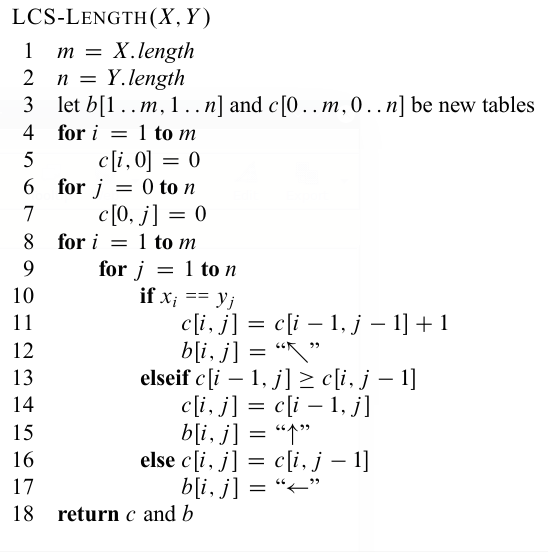
\includegraphics[width=0.5\linewidth]{imagenes/LCS.png}
        \caption{Algoritmo LCS (Cormen, pag. 394)}
        \label{fig:lcs}
    \end{figure}

    Ahora bien, tenemos dos ciclos que son lineales $\Theta(m)$ y $\Theta(n)$ en 
    las líneas $4 - 7$; pero en las líneas $8 - 17$ tenemos dos ciclos anidados 
    (para encontrar la $LCS$) lo que hace que tengan una complejidad de 
    $\Theta(mn)$, donde $n$ y $m$ son las longitudes de las secuencias. Así, 
    este algoritmo nos toma $\Theta(mn)$ tiempo en total.

    Por lo tanto, podemos aplicar este algoritmo para encontrar la longitud de 
    la subsecuencia más larga entre $S_1$ y $S_2$ en tiempo
    $\Theta(n \times n) = \Theta(n^2)$.

\end{enumerate}
\end{document}
